\documentclass[conference]{IEEEtran}

\usepackage{cite}
\usepackage{graphicx}
\usepackage{url}
\usepackage{booktabs}

\title{AI-Powered Kinyarwanda Educational Video Translation}

\author{%
\IEEEauthorblockN{Stephen N'nouka A. Issah, Wanchi Lucia Yen, Abduwaliyi Damilola Jimoh, Onitsiky Ranaivoson}
\IEEEauthorblockA{Carnegie Mellon University\\
AI System Design, Spring 2026\\
nnnoukaa@andrew.cmu.edu, wluciaye@andrew.cmu.edu, ajimoh@andrew.cmu.edu, oranaivo@andrew.cmu.edu}
}

\begin{document}

\pagestyle{plain}

\maketitle

\begin{abstract}
This report presents an AI system for translating short English educational videos into Kinyarwanda using automatic speech recognition, neural machine translation, and speech synthesis. The project targets SDG 4 (Quality Education) and SDG 10 (Reduced Inequalities) by reducing language barriers for learners who benefit from localized instructional content. Our deployed system accepts videos up to 3 minutes and 10 MB, uploads them through a signed-URL workflow, polls for Amazon Transcribe outputs, converts token-level transcripts into sentence segments, translates each segment with an NLLB-based model, synthesizes Kinyarwanda audio with DeepKIN FlexKinyaTTS, and plays the generated speech over a muted video in a web interface. On the language-modeling side, we cleaned and combined Digital Umuganda and MbazaNLP educational corpora, producing 44,979 general-domain pairs and 57,342 training-domain pairs after filtering. Offline fine-tuning experiments on NLLB-200 delivered a strong baseline and modest gains after domain-weighted adaptation, improving held-out test BLEU from 44.57 to 44.68 and ChrF from 70.44 to 70.46 while converging to a validation loss near 0.71. The main contribution of the project is therefore system integration: turning multilingual research artifacts into a working educational dubbing pipeline with explicit runtime limits, recoverable job states, cloud storage orchestration, and a low-cost hybrid deployment path that is realistic for a course-scale production demo.
\end{abstract}

\section{Introduction and SDG Relevance}
Educational video is abundant online, but most high-quality content remains inaccessible to learners who prefer or require local languages. This problem is especially important for Kinyarwanda-speaking audiences, where the digital education ecosystem is growing faster than the supply of localized video narration. Our project addresses this gap with an AI-assisted dubbing system that translates English educational videos into Kinyarwanda while preserving segment timing and playback continuity.

The work aligns with SDG 4 by improving access to learning materials and with SDG 10 by reducing linguistic inequality in digital education~\cite{un_sdg,unesco_mother_tongue}. Rather than treating translation as a standalone NLP task, we frame the problem as an AI systems design challenge: the system must ingest media, coordinate cloud services, transform transcript structure, run language models, synthesize speech, and expose outputs through a usable interface.

Our final implementation focuses on short-form instructional content suitable for demos and constrained deployment. The system does not yet export a permanently remixed dubbed video; instead, it produces timestamped Kinyarwanda audio segments and synchronizes them against muted video during playback in the browser. This choice keeps the system operationally simple while still demonstrating a full end-to-end localized learning experience.

\section{Related Work}
The project draws from three lines of prior work: massively multilingual translation, speech-enabled education pipelines, and language technologies for low-resource African languages.

For machine translation, we build on No Language Left Behind (NLLB), a multilingual sequence-to-sequence model designed to improve translation quality for low-resource languages at scale~\cite{nllb}. NLLB is a strong fit because Kinyarwanda is included in the supported language inventory and the model can be adapted through domain-weighted fine-tuning. We evaluate translation quality with BLEU and ChrF using SacreBLEU, following standard reproducible MT practice~\cite{sacrebleu}.

For speech processing, the deployed system uses Amazon Transcribe as the upstream ASR service to convert uploaded media into timestamped transcript artifacts in S3~\cite{aws_transcribe}. This decision shifts the project from a notebook-only prototype to a production-oriented cloud workflow with storage events, polling, and recoverable failures.

For Kinyarwanda speech generation, we use DeepKIN FlexKinyaTTS, a specialized TTS stack for Kinyarwanda text normalization and waveform synthesis~\cite{deepkin_repo}. This is important because generic multilingual TTS options often underperform on pronunciation, morphology, or prosody for low-resource languages. Our system therefore combines a global translation backbone with a language-specific speech model.

\section{Methodology}
\subsection{System Overview}
The deployed architecture is shown conceptually in Fig.~\ref{fig:architecture}. A React frontend handles file validation, job polling, and segment playback in the browser. A FastAPI backend validates uploads, manages job state, uploads videos to S3 through a signed-URL service, waits for transcript JSON, translates sentence segments, synthesizes audio, stores artifacts in S3, and returns a manifest consumed by the frontend. The result is a hybrid system: client-side code handles media interaction and synchronized playback, while cloud services and backend inference handle storage, ASR, translation, and TTS.

\begin{figure}[t]
\centering
\fbox{\parbox{0.95\columnwidth}{\small
Frontend upload $\rightarrow$ signed URL $\rightarrow$ S3 input $\rightarrow$ Lambda trigger $\rightarrow$ Amazon Transcribe $\rightarrow$ transcript JSON $\rightarrow$ FastAPI sentence segmentation $\rightarrow$ NLLB translation $\rightarrow$ DeepKIN TTS $\rightarrow$ public S3 audio + manifest $\rightarrow$ React playback over muted video.
}}
\caption{Deployed end-to-end architecture for educational video localization.}
\label{fig:architecture}
\end{figure}

Backend job states are explicit: \texttt{queued}, \texttt{processing}, \texttt{completed}, and \texttt{failed}. The API also records stage-level progress such as \texttt{upload\_video}, \texttt{wait\_transcript}, \texttt{translate\_and\_tts}, and \texttt{upload\_manifest}. This design was chosen so that failures after upload can be resumed without re-running the full pipeline.

\subsection{Datasets and Preprocessing}
The translation component uses two parallel corpora downloaded from Kaggle: Digital Umuganda, a larger general-domain English-Kinyarwanda corpus, and MbazaNLP, an education-focused corpus with train, validation, and test splits~\cite{digital_umuganda,mbaza}. We normalized whitespace and punctuation, removed empty rows, deduplicated sentence pairs, filtered sentence lengths outside 2--100 words, and removed examples with extreme Kinyarwanda-to-English length ratios.

Table~\ref{tab:data} summarizes the retained data. Cleaning was most impactful on Digital Umuganda because it contained 2,376 duplicate rows and small amounts of missing data. MbazaNLP was already comparatively clean. The cleaned corpora reveal a consistent structural pattern: Kinyarwanda sentences are shorter in word count than English sentences on average, reflecting the language's richer morphology.

\begin{table}[t]
\centering
\caption{Dataset summary after preprocessing.}
\label{tab:data}
\begin{tabular}{lrrr}
\toprule
Split & Raw & Cleaned & Retained \\
\midrule
Digital Umuganda & 47,824 & 44,979 & 94.1\% \\
Mbaza Train & 58,251 & 57,342 & 98.4\% \\
Mbaza Val & 2,456 & 2,402 & 97.8\% \\
Mbaza Test & 1,060 & 1,048 & 98.9\% \\
\bottomrule
\end{tabular}
\end{table}

The cleaned sentence statistics also show the domain shift we had to manage. Digital Umuganda averages 6.15 Kinyarwanda words and 8.54 English words per example, while Mbaza Train averages 13.40 Kinyarwanda words and 17.74 English words. This confirms that general web text alone is insufficient for classroom-style language.

\subsection{Translation Model}
We used \texttt{facebook/nllb-200-distilled-600M} as the base translation model~\cite{nllb}. The tokenizer and model were configured for \texttt{eng\_Latn} to \texttt{kin\_Latn}. Training used domain-weighted data mixing: every cleaned Mbaza training example appeared twice, and a size-matched sample of cleaned Digital Umuganda examples was added once. Because the general corpus sample size was capped at the smaller of the two corpora, the final training set contained 159,663 parallel pairs: 114,684 education-weighted examples and 44,979 general-domain examples.

Fine-tuning settings extracted from the notebook were: learning rate $2\times10^{-5}$, per-device batch size 4, gradient accumulation 4 (effective batch size 16), maximum sequence length 128, and 3 epochs. The training history artifact records 29,937 optimization steps, a final average train loss of 3.14, total training runtime of 21,785.85 seconds (about 6.05 hours), training throughput of 21.99 samples/s, and validation loss that decayed to roughly 0.71.

The research and deployment configurations are intentionally separated. Offline experiments produced a fine-tuned checkpoint for evaluation, but the deployable backend exposes the translation model through an environment variable and currently defaults to the base NLLB model name. This keeps the deployed service simpler to bootstrap while preserving a clean path to swap in the fine-tuned checkpoint later.

\subsection{Speech and Playback Pipeline}
The upstream speech recognition stage is externalized. Videos are uploaded to S3, an AWS Lambda starts an Amazon Transcribe job, and the backend later polls for the transcript artifact. Transcript tokens are then grouped into sentence-level segments by detecting punctuation boundaries in Transcribe-style \texttt{results.items}. Each sentence is translated and converted into a standalone WAV file using DeepKIN FlexKinyaTTS.

Instead of muxing audio back into a final MP4, the current deployed frontend mutes the original video and schedules the generated audio clips using each segment's \texttt{start\_time}. This is an intentional systems tradeoff: synchronized browser playback is cheaper and faster to iterate on than server-side remastering, while still demonstrating the user-facing learning experience.

\section{Experiments and Evaluation}
\subsection{Data Quality Analysis}
Fig.~\ref{fig:cleaning} shows the effect of cleaning on corpus size and average sentence length. The largest absolute reduction occurred in Digital Umuganda, while MbazaNLP splits were only lightly pruned. Fig.~\ref{fig:lengths} confirms that the domain-specific corpus is both longer and more variable than the general corpus, supporting our decision to up-weight Mbaza examples during fine-tuning.

\begin{figure}[t]
\centering
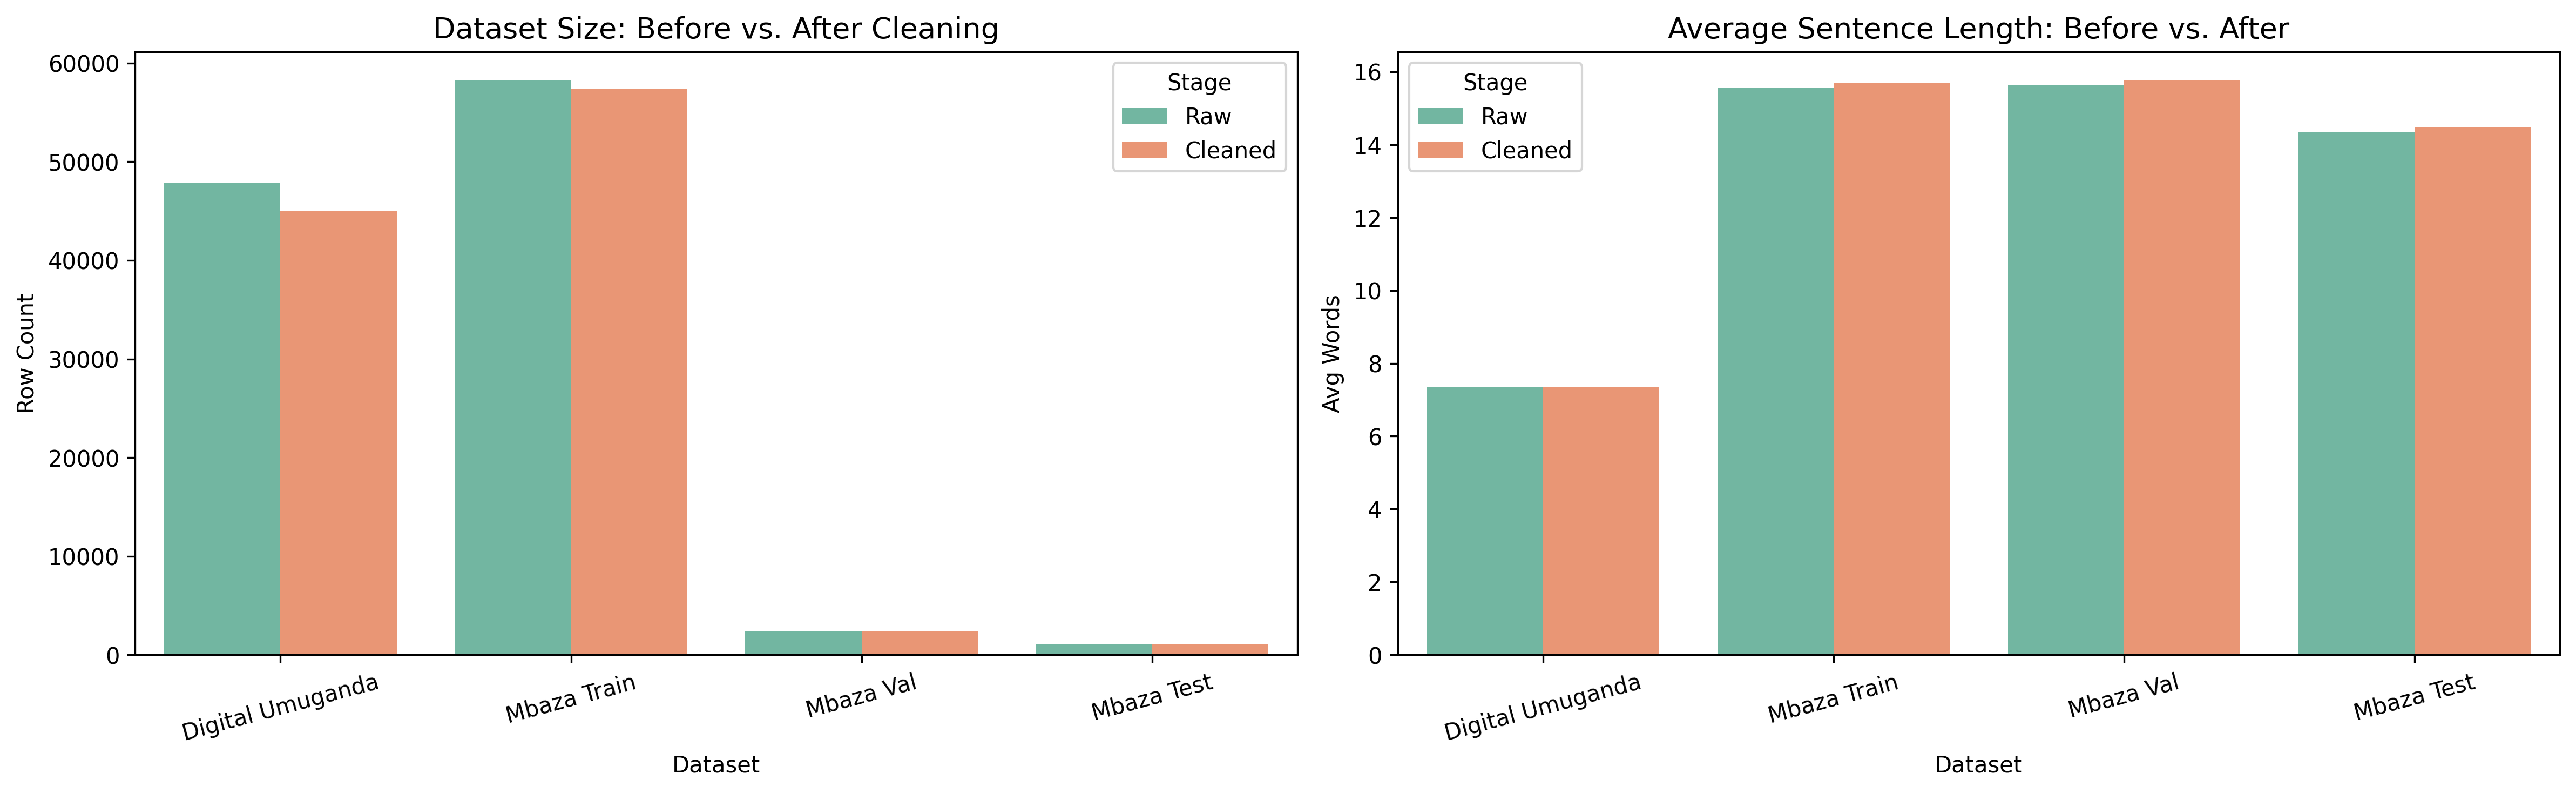
\includegraphics[width=\columnwidth]{cleaning_comparison.png}
\caption{Rows retained and average sentence length before and after preprocessing.}
\label{fig:cleaning}
\end{figure}

\begin{figure}[t]
\centering
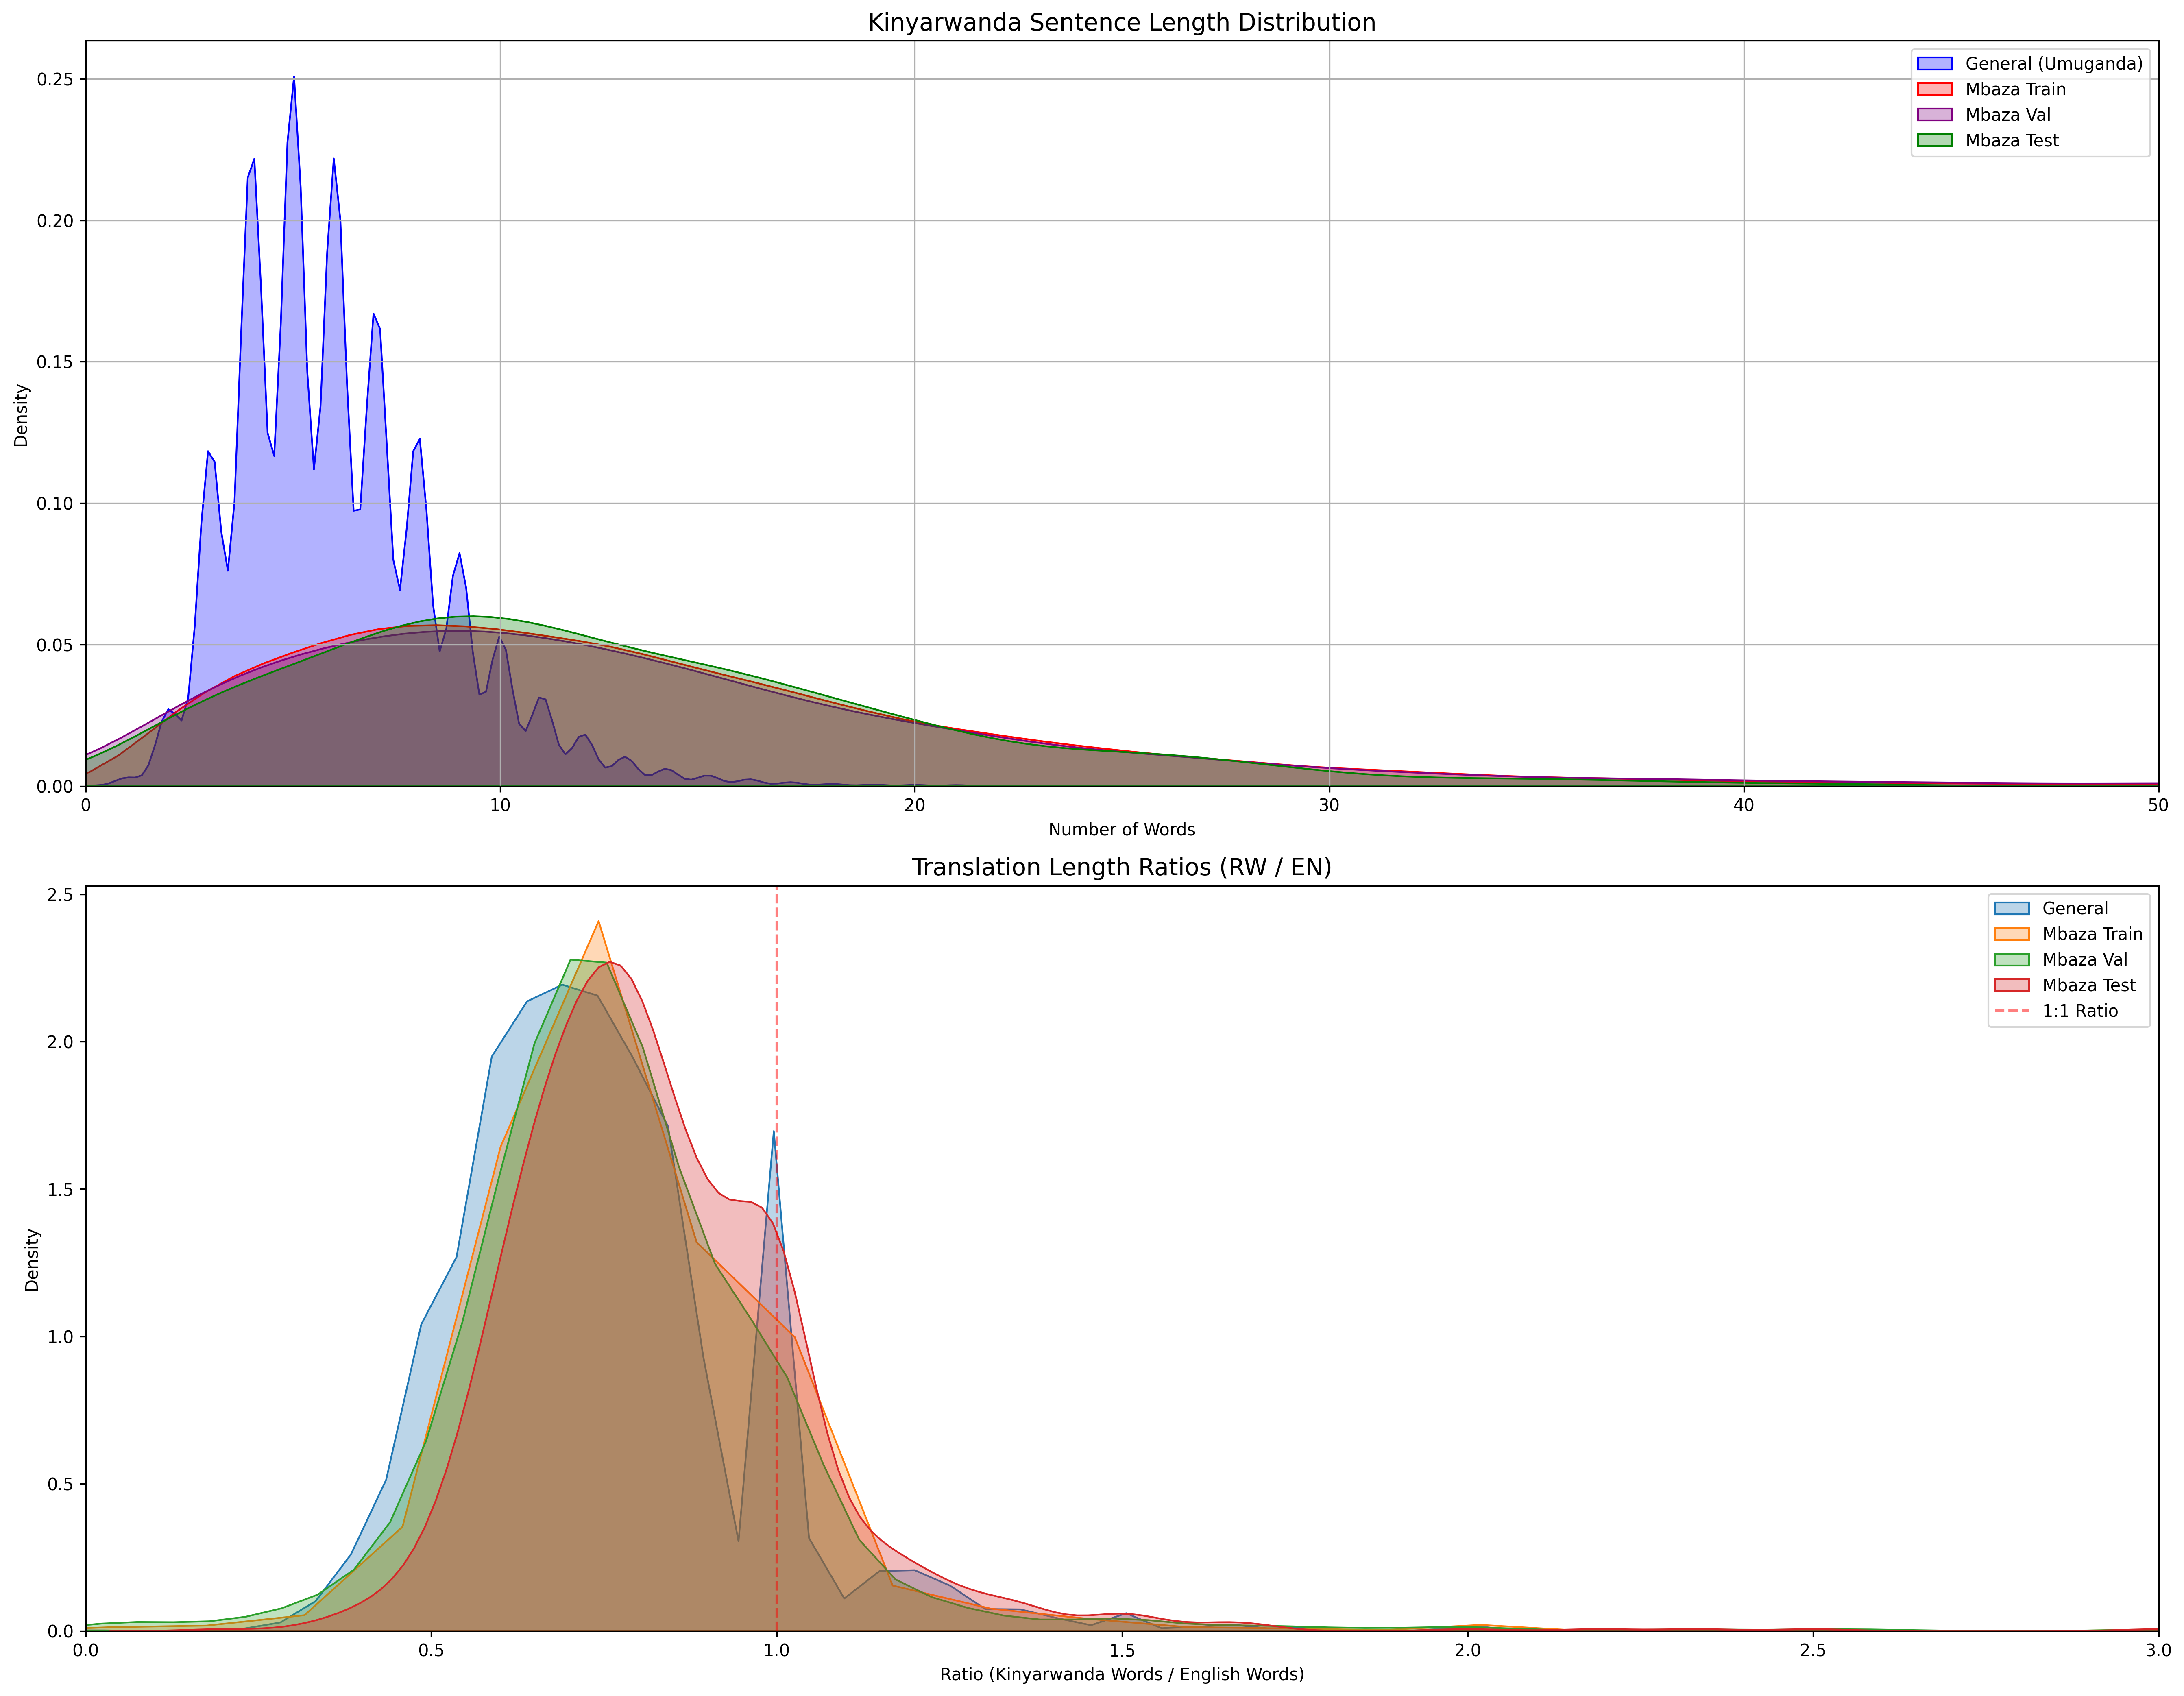
\includegraphics[width=\columnwidth]{sentence_length_distribution.png}
\caption{Sentence length and Kinyarwanda-to-English length ratio distributions across corpora.}
\label{fig:lengths}
\end{figure}

\subsection{Translation Metrics}
The pretrained model was first evaluated on a 200-sample validation subset, where it achieved BLEU 15.73 and ChrF 50.83. This already met the course target of ChrF above 50, indicating that NLLB provides a strong low-resource baseline before any task-specific adaptation.

Held-out test evaluation used 100 samples from the cleaned Mbaza test split. Results are shown in Table~\ref{tab:metrics}. Fine-tuning improved BLEU by 0.11 and ChrF by 0.02. These gains are small but positive. This comparison serves as our lightweight ablation: pretrained multilingual transfer is already strong, and domain-weighted fine-tuning helps, but only modestly, under the available data and compute budget.

\begin{table}[t]
\centering
\caption{Translation quality on held-out Mbaza test samples.}
\label{tab:metrics}
\begin{tabular}{lrrr}
\toprule
Metric & Baseline & Fine-tuned & $\Delta$ \\
\midrule
BLEU & 44.57 & 44.68 & +0.11 \\
ChrF & 70.44 & 70.46 & +0.02 \\
\bottomrule
\end{tabular}
\end{table}

Notebook error analysis still revealed useful qualitative improvements on selected examples, especially where education-specific phrasing benefited from weighted exposure. However, several low-BLEU errors remained tied to morphology, rare terminology, or copied English fragments, suggesting that future improvements will depend more on data expansion and human review than on simply extending the same fine-tuning recipe.

\subsection{Training Dynamics and Resource Use}
Fig.~\ref{fig:training} plots training and validation loss with the linear learning-rate schedule. The validation curve stabilizes early and remains flat after the initial drop, which is consistent with the marginal test-set gains. By step 29,500, evaluation loss had reached 0.7111, and the final training summary recorded 1.37 optimizer steps/s. In other words, training converged cleanly, but the bottleneck was data and domain coverage rather than optimization instability.

For deployment planning, model artifact sizes are significant. The packaged DeepKIN checkpoint in the deployable workspace is 1.035 GB, and notebook logs show that the NLLB-200 model download includes a \texttt{model.safetensors} file of approximately 2.46 GB. These sizes matter for cold start time, storage provisioning, and whether models are baked into images or pulled at runtime.

\begin{figure}[t]
\centering
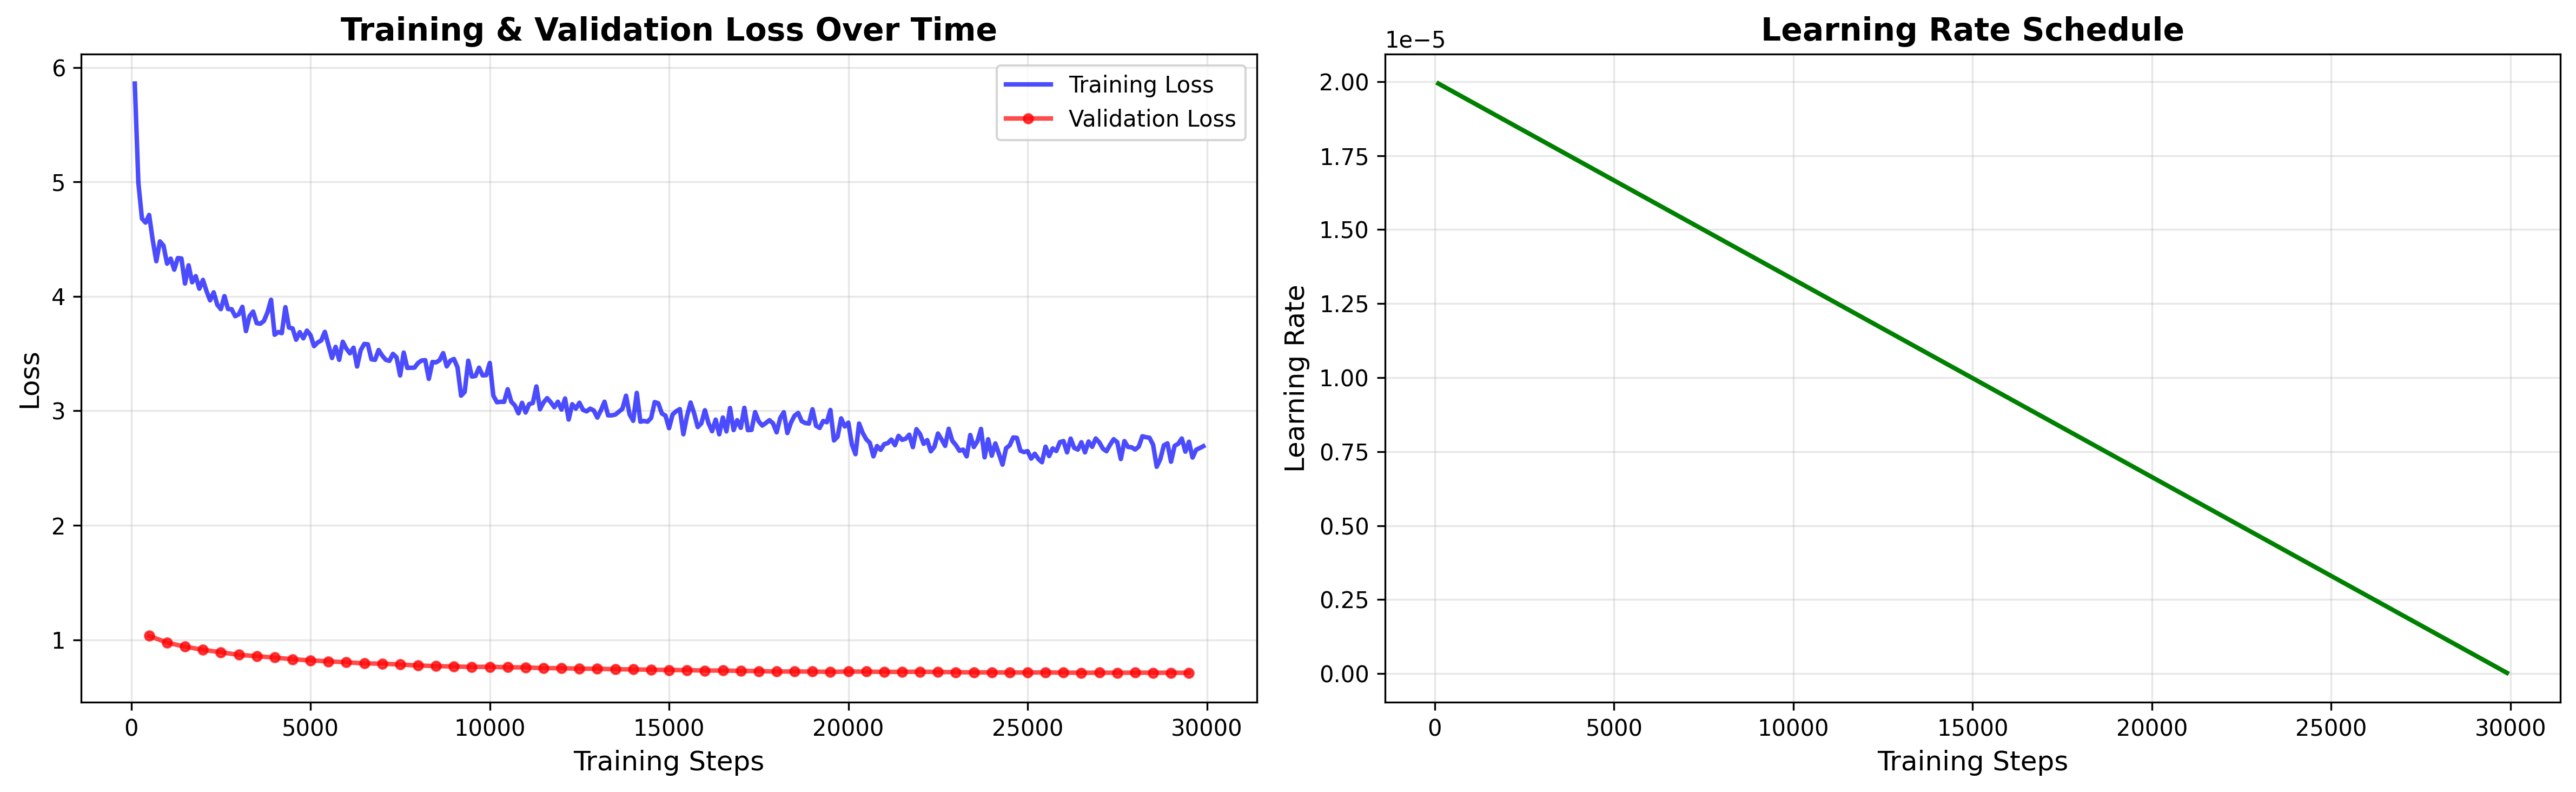
\includegraphics[width=\columnwidth]{training_history_plot.png}
\caption{Training loss, validation loss, and learning-rate schedule for NLLB fine-tuning.}
\label{fig:training}
\end{figure}

\section{Deployment and Scalability}
The deployable system is split into a static frontend and a containerized backend. The frontend is a React + Vite single-page application that can be hosted on S3 and distributed through CloudFront. The backend is a FastAPI service that can run locally with Docker or in the cloud on ECS, Fargate, EKS, or EC2. The deployment guide also documents a budget-oriented EC2 option using \texttt{t3.medium} or \texttt{t4g.medium} with an estimated cost near \$30 per month.

Table~\ref{tab:deployment} makes the edge-cloud-hybrid design explicit. Browser code performs local validation, timed playback, and user interaction; AWS services provide durable storage and ASR; and the backend container performs translation, TTS, and job orchestration. This partitioning keeps the public interface lightweight while centralizing the heavier ML inference and storage responsibilities.

\begin{table}[t]
\centering
\caption{Hybrid deployment responsibilities and scaling constraints.}
\label{tab:deployment}
\footnotesize
\begin{tabular}{p{0.18\columnwidth}p{0.20\columnwidth}p{0.54\columnwidth}}
\toprule
Component & Placement & Role / constraint \\
\midrule
Upload and playback & Browser edge & Enforces 10 MB and 180 s limits, polls job state, and schedules translated audio over muted video. \\
Storage and ASR & AWS cloud & Uses signed S3 uploads, Lambda-triggered transcription, 5 s polling, and a 600 s transcript timeout. \\
Translation and TTS & Backend container & Loads NLLB and DeepKIN, runs asynchronous jobs, and is currently executed with a 2-worker thread pool. \\
Job metadata & Local persistent volume & Stores recoverable job state in SQLite; acceptable for demo scale but not ideal for many concurrent users. \\
\bottomrule
\end{tabular}
\normalsize
\end{table}

Operational safeguards are built into both the client and server. Uploaded videos are limited to 10 MB and 180 seconds. The transcript polling interval is 5 seconds with a 600-second timeout. Backend health and readiness endpoints expose model availability, and Nginx is recommended as a reverse proxy so the application port remains private in production. SQLite is used for job metadata in the current prototype, which is acceptable for course-scale demos but would likely need to be replaced with a managed store for concurrent multi-user deployment.

From a scalability perspective, the most expensive stages are transcript generation, translation model loading, and TTS waveform synthesis. The current architecture can be improved by caching translation outputs, batching TTS requests, preloading model weights on worker startup, and replacing SQLite with a managed job store. Even without these optimizations, the pipeline demonstrates an important design principle: low-cost cloud primitives plus model artifacts can support a usable localized learning workflow without requiring a full MLOps stack.

\section{Responsible AI and Ethical Considerations}
The primary ethical risk is overtrust in generated educational content. A mistranslated instructional sentence or incorrectly synthesized term can mislead learners, especially when the system is used for foundational subjects. This risk is amplified in low-resource settings where users may not have an easy way to verify the English source.

We address this partially through system design choices. First, the frontend exposes segment-level text and timing rather than hiding model outputs behind a single opaque audio stream. Second, the backend surfaces explicit failure states instead of silently dropping segments. Third, the training data was cleaned to reduce malformed or mismatched sentence pairs. These steps improve transparency, but they do not eliminate linguistic bias or hallucination.

There are also privacy and security concerns. Video uploads may contain children, classrooms, or copyrighted content. Earlier browser-based transcription prototypes required AWS credentials directly in the client, which is appropriate only for demos. The deployable stack is safer because uploads are mediated through backend-managed signed URLs, but storage retention, access control, and consent policies still need to be formalized before any real-world deployment.

Finally, the voice output raises representation questions. A single TTS voice cannot reflect the diversity of Kinyarwanda speakers, dialectal preferences, or age-appropriate narration styles. Future versions should include speaker selection, native-speaker evaluation, and human review workflows for high-stakes educational use.

\section{Results and Discussion}
The strongest result of the project is not a large jump in MT metrics; it is the successful composition of multiple AI and cloud components into a coherent educational localization system. The translation model remained strong after domain adaptation, the TTS stage produced segment-level Kinyarwanda audio, and the deployed frontend demonstrated synchronized dubbing of uploaded educational videos using real cloud artifacts.

The quantitative findings are mixed but still informative. The corpus analysis justified domain weighting, yet test-set gains after fine-tuning were small. This suggests that for English-to-Kinyarwanda educational translation, system quality may now be constrained less by model architecture and more by data coverage, terminology alignment, and end-user evaluation. Put differently, the project shifted the bottleneck from ``Can the model translate at all?'' to ``Can the full system translate reliably enough for instruction?''

This is a useful systems-design outcome. It means future effort should focus on targeted corpus expansion, human evaluation with educators or native speakers, glossary constraints for key educational terminology, and tighter playback synchronization rather than repeating the same training recipe. The project therefore surfaces a realistic product lesson: in applied AI systems, integration, UX, and operational safety often matter as much as marginal benchmark improvement. It also clarifies a near-term engineering task for this codebase: wiring the validated fine-tuned checkpoint into the production backend without sacrificing startup time or deployment simplicity.

\section{Conclusion and Future Work}
We built and deployed an AI-powered Kinyarwanda educational video translation system that combines cloud transcription, NLLB-based translation, DeepKIN speech synthesis, and a web playback interface. The system operationalizes SDG-oriented language access by turning short English videos into synchronized Kinyarwanda audio experiences. Our experiments showed that the pretrained translation baseline was already strong and that domain-weighted fine-tuning yielded only small metric gains, while the broader pipeline integration delivered the main practical value.

Future work should focus on four areas: larger education-specific parallel corpora, native-speaker human evaluation, server-side export of dubbed MP4 files, and stronger production safeguards for storage, consent, and monitoring. With those additions, the prototype can evolve from a course project into a more robust platform for multilingual educational delivery.

\bibliographystyle{IEEEtran}
\bibliography{references}

\end{document}
